\section{Que es la regresión lineal multiple}

La regresión lineal múltiple es una extensión de la regresión lineal simple. Ambas son técnicas de análisis estadístico que modelan la relación entre una variable dependiente y una o más variables independientes.
Gracias a esta regresión se pueden modelar relaciones mas complejas y considerando mas variables, pero es mas complejo de hacer

\section{Metodología}
Usamos las siguientes importaciones para el programa
\begin{figure}[h]
    \centering
    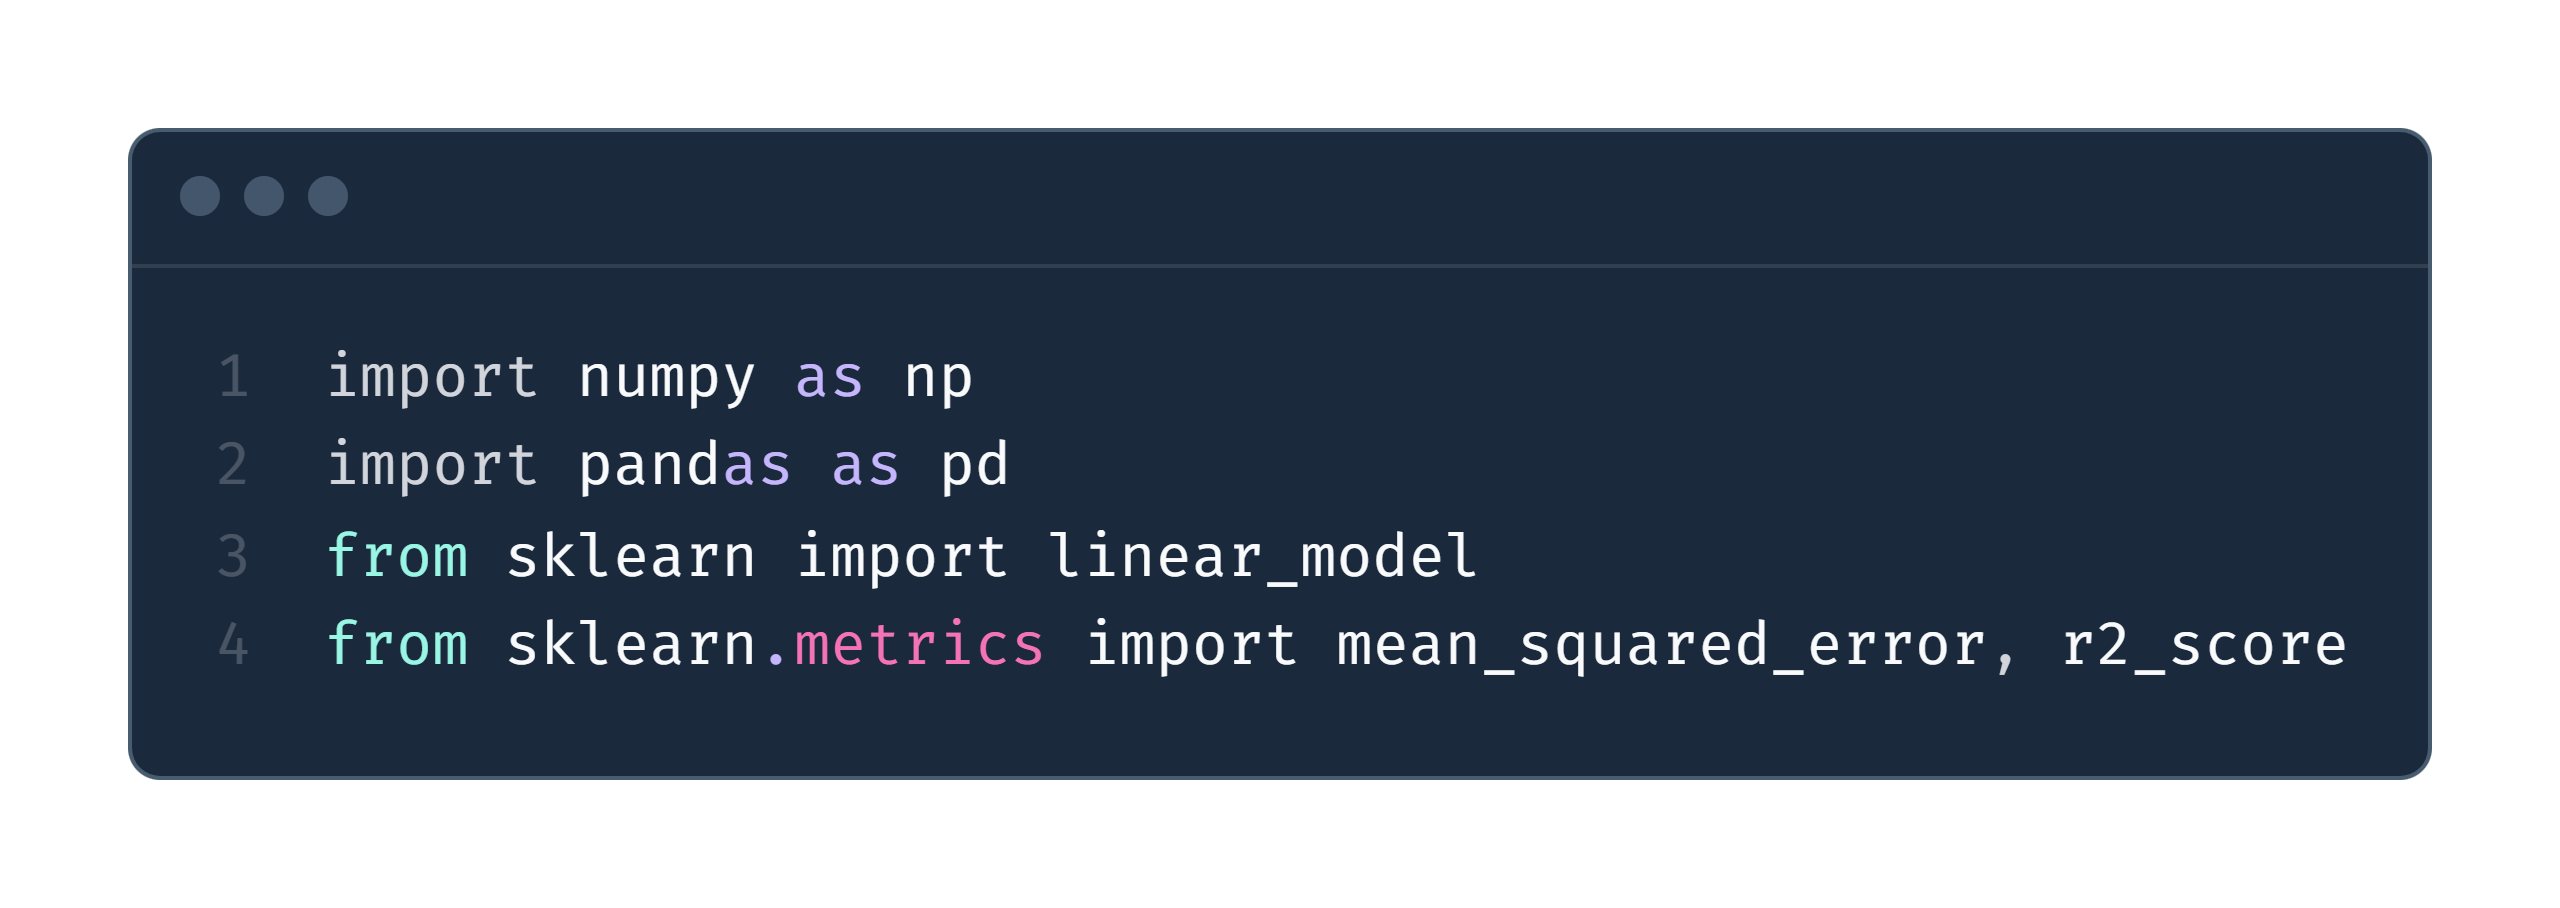
\includegraphics[width=0.5\linewidth]{image.png}
\end{figure}
Ademas, agregamos el código necesario al programa que se hizo anteriormente de regresión lineal ya que este es una mejora del anterior
\begin{figure}[h]
    \centering
    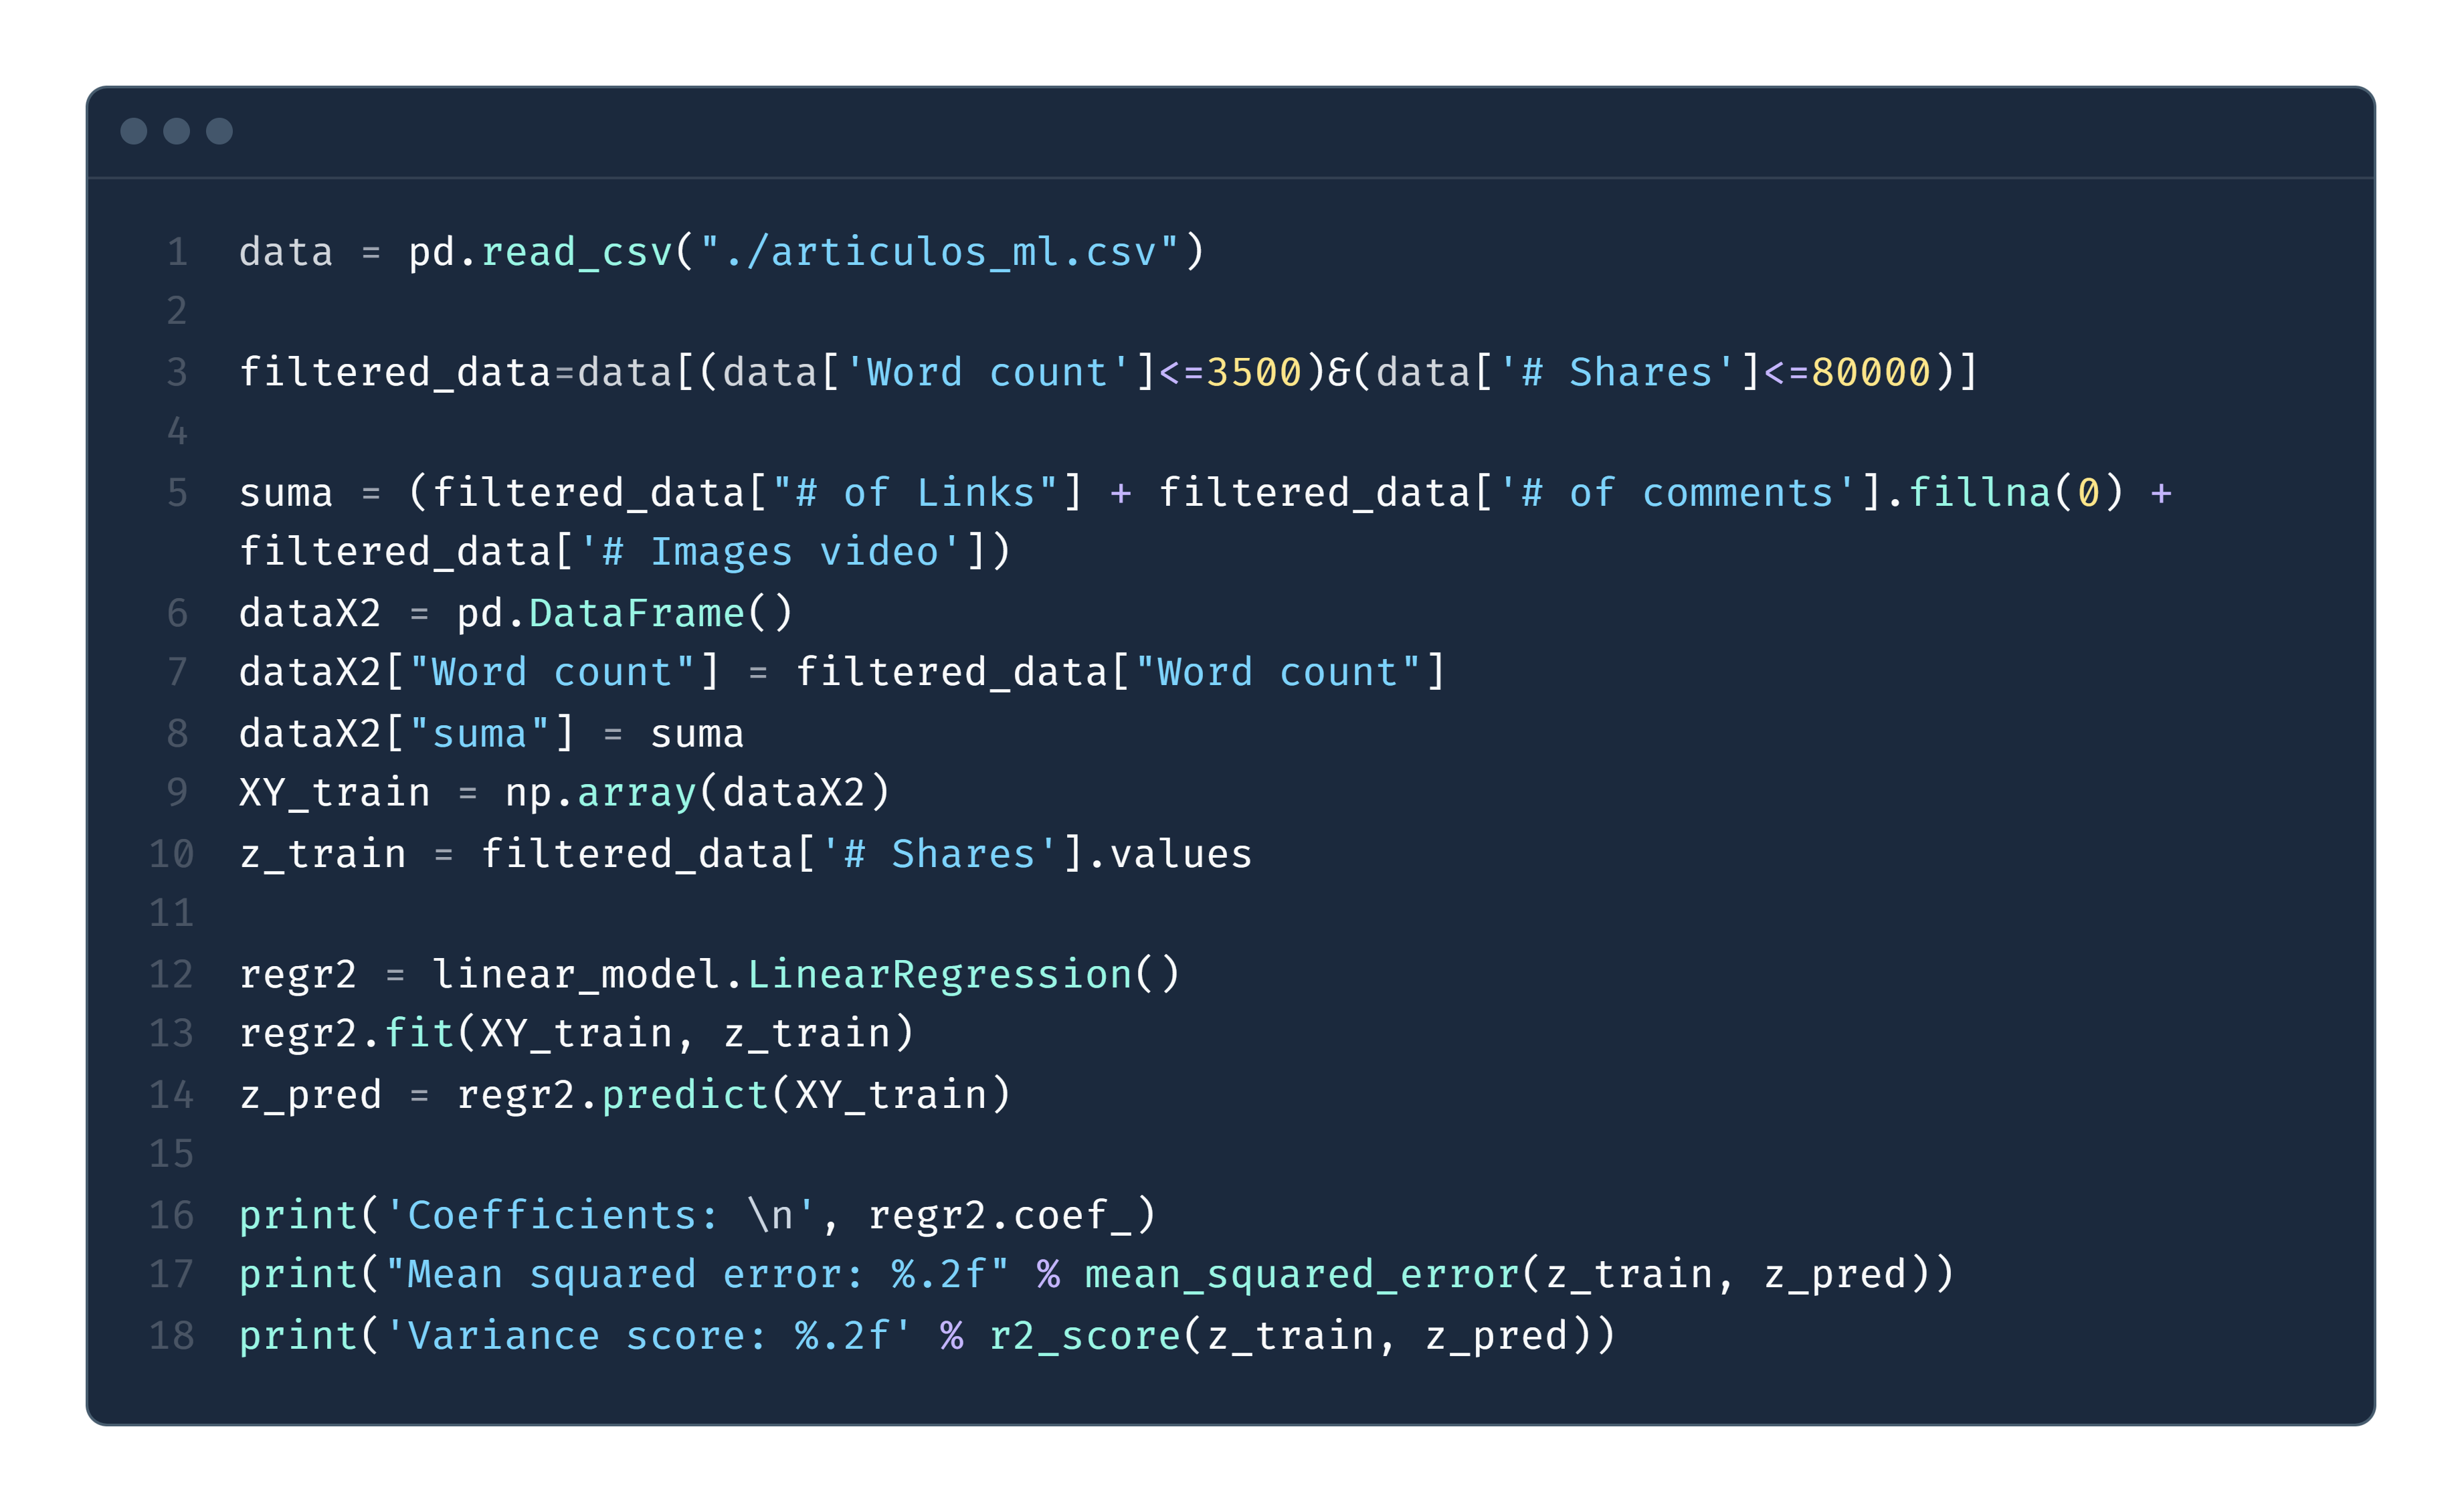
\includegraphics[width=0.5\linewidth]{image_2.png}
\end{figure}
A diferencia del programa anterior ahora tomaremos en cuenta una variable suma que es la combinación de la cantidad de enlaces, comentarios, imágenes y videos en el articulo.


\section{Resultados}
Al ejecutar el programa obtenemos los siguientes valores
\begin{table}[h]
    \centering
    \begin{tabular}{|c|c|} \hline 
        Coefficients & [$6.63$,$-483.41$]\\ \hline 
        Mean squared error& $352122816.48$\\ \hline 
        Variance score& $0.11$\\\hline
    \end{tabular}
\end{table}


\section{Conclusión}
Si bien el modelo mejoro ligeramente no fue suficiente, el error cuadrático sigue siendo muy elevado y el coeficiente de determinación es igualmente muy bajo.
Es necesario tomar en cuanta mas variables o volver a pensar en como esta modelado este problema